In the quest to uncover the mysteries of Valyrian steel and its extraordinary properties, we often find ourselves intrigued by the elegant curves and contours of Valyrian steel swords. These unique blade shapes not only contribute to the aesthetic allure of these legendary weapons but may also play a crucial role in their functionality. In this appendix, we provide Python code that demonstrates how to fit a curve to the curvature of a Valyrian steel sword.

This Python code leverages the SciPy library to fit a curve to the curvature data of a Valyrian steel sword. The \text{sword\_curve} function represents the hypothesized curve, and the \text{curve\_fit} function optimizes the parameters to best fit the data. The resulting parameters \text{a\_opt},\text{b\_opt}, and \text{c\_opt} describe the curve's shape.

Remember to replace the sample data with actual measurements if available. This code serves as a starting point for analyzing and characterizing the curvature of Valyrian steel swords, contributing to our understanding of these legendary weapons' craftsmanship and functionality.

\begin{figure} [H]
    \centering
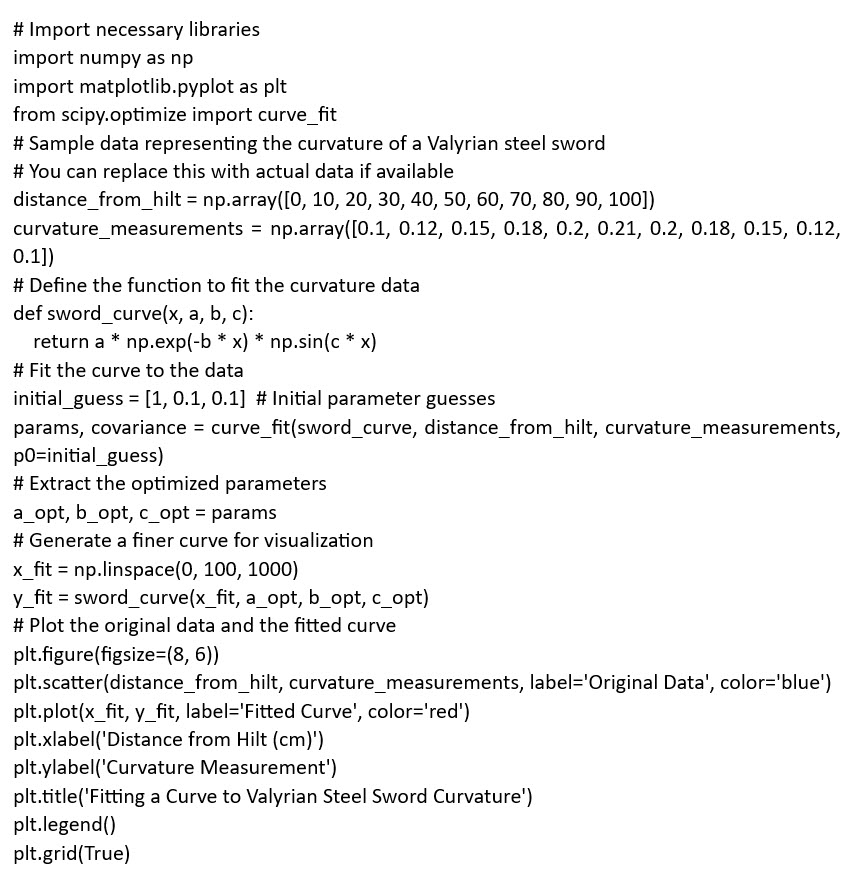
\includegraphics{images/python.jpg}
    \caption{Python code used to .....}
    \label{fig:python}
\end{figure}

